\section{Selecting bets for a rejection horizon}
\label{sec:lambda-power}
The optimizer $\delta/(2\nu^2)$ in T2 maximizes its inverse-capital power
certificate. It need not maximize actual crossing probability. Two other
objectives are expected log-evidence growth and rejection before a specified
deadline. They generally select different bets. The capital in this section
is statistical evidence, not investible fund wealth.

\subsection{Expected log growth has a different optimizer}
For a fixed conditional score law with mean $\delta$ and
$\E Y^2\le\nu^2$, write
\[
 g_{\log}(\lambda)=\E\phi(\lambda Y)-\lambda^2\nu^2/2.
\]
\begin{proposition}[A strictly concave log-growth objective]
The function $g_{\log}$ is strictly concave on $[0,\infty)$, with
\[
 -\frac54\nu^2\le g_{\log}''(\lambda)\le-\frac34\nu^2.
\]
If $\delta\le0$, its nonnegative maximizer is zero. If $\delta>0$, its
unconstrained maximizer is the unique solution of
\begin{equation}
 \E\!\left[Y\frac{1+\lambda|Y|}
 {1+\lambda|Y|+\lambda^2Y^2/2}\right]=\lambda\nu^2,
 \qquad
 \frac{4\delta}{5\nu^2}\le\lambda_{\log}^*
 \le\frac{4\delta}{3\nu^2}.\label{eq:log-optimal-bet}
\end{equation}
A finite upper cap clips this maximizer.
\end{proposition}
\begin{proof}
Differentiating the specified Catoni function gives
\[
 \phi'(x)=\frac{1+|x|}{1+|x|+x^2/2},\qquad
 \phi''(x)=-\operatorname{sign}(x)
 \frac{|x|+x^2/2}{(1+|x|+x^2/2)^2}.
\]
The second derivative extends continuously by zero at the origin.
Setting $u=1+|x|$ shows that $|\phi''(x)|$ is bounded by the maximum of
$2(u^2-1)/(u^2+1)^2$, namely $1/4$. Finite $\E Y^2$ permits dominated
differentiation. Thus $g_{\log}''=\E[Y^2\phi''(\lambda Y)]-\nu^2$ has the
stated bounds. Its derivative at zero is $\delta$ and decreases strictly
to a negative value. Integrating the derivative bounds proves
\eqref{eq:log-optimal-bet} and the capped result.
\end{proof}

For small transformed scores, $\lambda_{\log}^*$ is near
$\delta/\nu^2$, rather than $\delta/(2\nu^2)$. Optimizing a fitted law
therefore targets \emph{predicted} log growth; it does not establish optimal
growth under an unknown true law. Nor does log-growth optimization solve a
finite-deadline power problem. These distinctions are compatible with the
existing general betting and log-optimality literature \cite{instance}.

\subsection{Targeting power directly}
Fix a working law for future score blocks, a finite action set
$\mathcal A\subset[0,\lambda_{\max}]$ containing zero, and
$b_\alpha=\log(1/\alpha)$. A constant bet within a block of $h$ scores has
working log-capital increment
\[
 Z_\lambda=\sum_{i=1}^h\phi(\lambda Y_i)-h\lambda^2\nu^2/2,
 \qquad Z_\lambda\sim Q_\lambda.
\]
Suppose the next block has this conditional working distribution given the
chosen action, independently of earlier blocks. Set
\begin{equation}
 V_0(\ell)=\mathbf1\{\ell\ge b_\alpha\},\qquad
 V_k(\ell)=
 \begin{cases}
 1,&\ell\ge b_\alpha,\\
 \displaystyle\max_{\lambda\in\mathcal A}
       \int V_{k-1}(\ell+z)Q_\lambda(dz),&\ell<b_\alpha.
 \end{cases}\label{eq:power-bellman}
\end{equation}
\begin{proposition}[Working-model horizon power: a specialization]
The recursion gives the largest probability, under the specified working
model and action class, of crossing at a review within $k$ remaining blocks.
A maximizing action chosen from the current log capital and remaining time
is predictable. Under the \emph{real} datewise null and real public moment
bound, the resulting process retains T1's individual type-I guarantee even
when the working power model is misspecified.
\end{proposition}
\begin{proof}
At zero remaining blocks the claim is the definition of crossing. At an
uncrossed state, condition on the next action and increment. The induction
hypothesis makes the conditional continuation value at most
$V_{k-1}(\ell+z)$; maximizing its integral gives the upper bound. Selecting a
maximizer and then the inductively optimal continuation attains it. The
finite action set permits measurable tie breaking. Each selected action uses
only pre-block information, so T1 applies separately to the real score law.
\end{proof}
This uses standard target reachability \cite{reachability}. More directly,
\cite{taga} studies horizon-aware bounded-mean betting, \cite{clerico} treats
rejection-time rewards and Bellman optimization, and \cite{baas} optimizes
finite-horizon binary-trial e-values. The recursion here is a specialization
to blockwise Catoni factors. The computed implementation also discretizes log capital; its numerical maximum
is not asserted to be a continuous-control global optimum. A full financial
score model would also need the evolving estimation and allocation states.
The scalar stationary calculation below does not supply that model.

\subsection{A separately frozen controlled comparison}
We fix the working score law at $N(.1,1)$, $\nu^2=1.09$,
$\alpha=.05$, and the common cap $1/(2\sqrt{1.09})$. Every rule keeps its bet
for 100 observations and can reject only at the same 100-observation reviews.
The declared deadlines are 400, 800 and 1600 observations. The fixed
certificate bet is $.0458716$ and the exact working-model log-growth bet is
$.0908020$. The horizon rule also uses its current capital and remaining
blocks; it is not a single larger constant bet.

Exact Gaussian CDF bins and FFT convolution give block-increment distributions.
The primary log-capital spacing is $.01$ with 129 regular actions; a refinement
uses $.005$, 257 actions and a wider lower boundary. Both include the fixed
comparison bets. Their predicted initial powers differ by at most $.000396$.
An initial nearest-grid implementation could round a real subthreshold capital
into the absorbing threshold state. The corrected lookup prevents this, and
the entire declared random stream is replayed without changing the numerical
grids, design alternative, cap or deadlines. Initial outputs remain diagnostics.

The evaluation uses 20,000 independent paths at each actual score mean
$0,.1,.2,.3$, all with variance one. All four laws satisfy the common public
moment bound. The actual mean determines only the generated scores; bets use
the fixed working law, pre-block capital and past scores. Mean zero checks the
boundary null; the other two non-design alternatives assess misspecification.
The following results concern this controlled score experiment, not additional
financial markets or a revised primary fund strategy.

\begin{table}[H]\centering\small

\begin{tabular}{lrrrrrr}

\toprule

& \multicolumn{3}{c}{Null rejection (\%)} & \multicolumn{3}{c}{Design power (\%)} \\

Rule & 400 & 800 & 1600 & 400 & 800 & 1600 \\

\midrule

Past-mean certificate & 0.11 & 0.22 & 0.32 & 11.41 & 37.76 & 78.29 \\

Fixed certificate & 0.02 & 0.19 & 0.96 & 4.00 & 44.94 & 93.04 \\

Fixed log growth & 0.69 & 1.44 & 1.98 & 28.31 & 66.50 & 92.44 \\

One-block power & 1.20 & 1.36 & 1.36 & 25.53 & 34.10 & 36.04 \\

Horizon DP & 1.42 & 1.84 & 2.25 & 37.48 & 72.83 & 97.07 \\

Refined horizon DP & 1.41 & 1.83 & 2.26 & 37.47 & 72.81 & 97.13 \\

\bottomrule\end{tabular}

\caption{Review-time rejection fractions from 20,000 paths per law. The null has mean zero and the design alternative mean .1, both with variance one. Every rule has the same individual nominal 5\% bound, public moment cap and bet/review calendar; observed null rates differ. Each horizon-DP entry uses a separate policy targeting that deadline.}\label{tab:lambda-power}\end{table}

At 400 observations the horizon rule crosses on 7496/20000 paths (37.48\%) versus 2281/20000 (11.41\%) for the past-mean rule. The paired difference is 26.08 percentage points (Monte Carlo 95\% interval [25.47, 26.68]). This compares a common nominal level, not matched actual null-crossing probabilities. At the longest deadline the fixed log-growth rule does not outperform the fixed certificate rule, illustrating that the objectives differ. The repeatedly greedy one-block rule also falls short of the deadline-specific policy.

The refined-grid powers closely agree with the primary implementation, and all six predicted-versus-observed design-power checks pass the declared numerical-plus-Monte-Carlo audit. All pre-block horizon-policy and fixed stakes, every first crossing, and the complete summary are independently reconstructed (12,331,336 scalar checks). Direct multiplicative score replay covers the first sixteen paths under each law; it is not a replay of every score path. Its maximum log-capital discrepancy is 6.17e-14. The stronger alternatives .2 and .3 are retained in the numeric report. No result supplies a power optimum for a changing financial score law or improved fund performance.

\begin{figure}[H]\centering

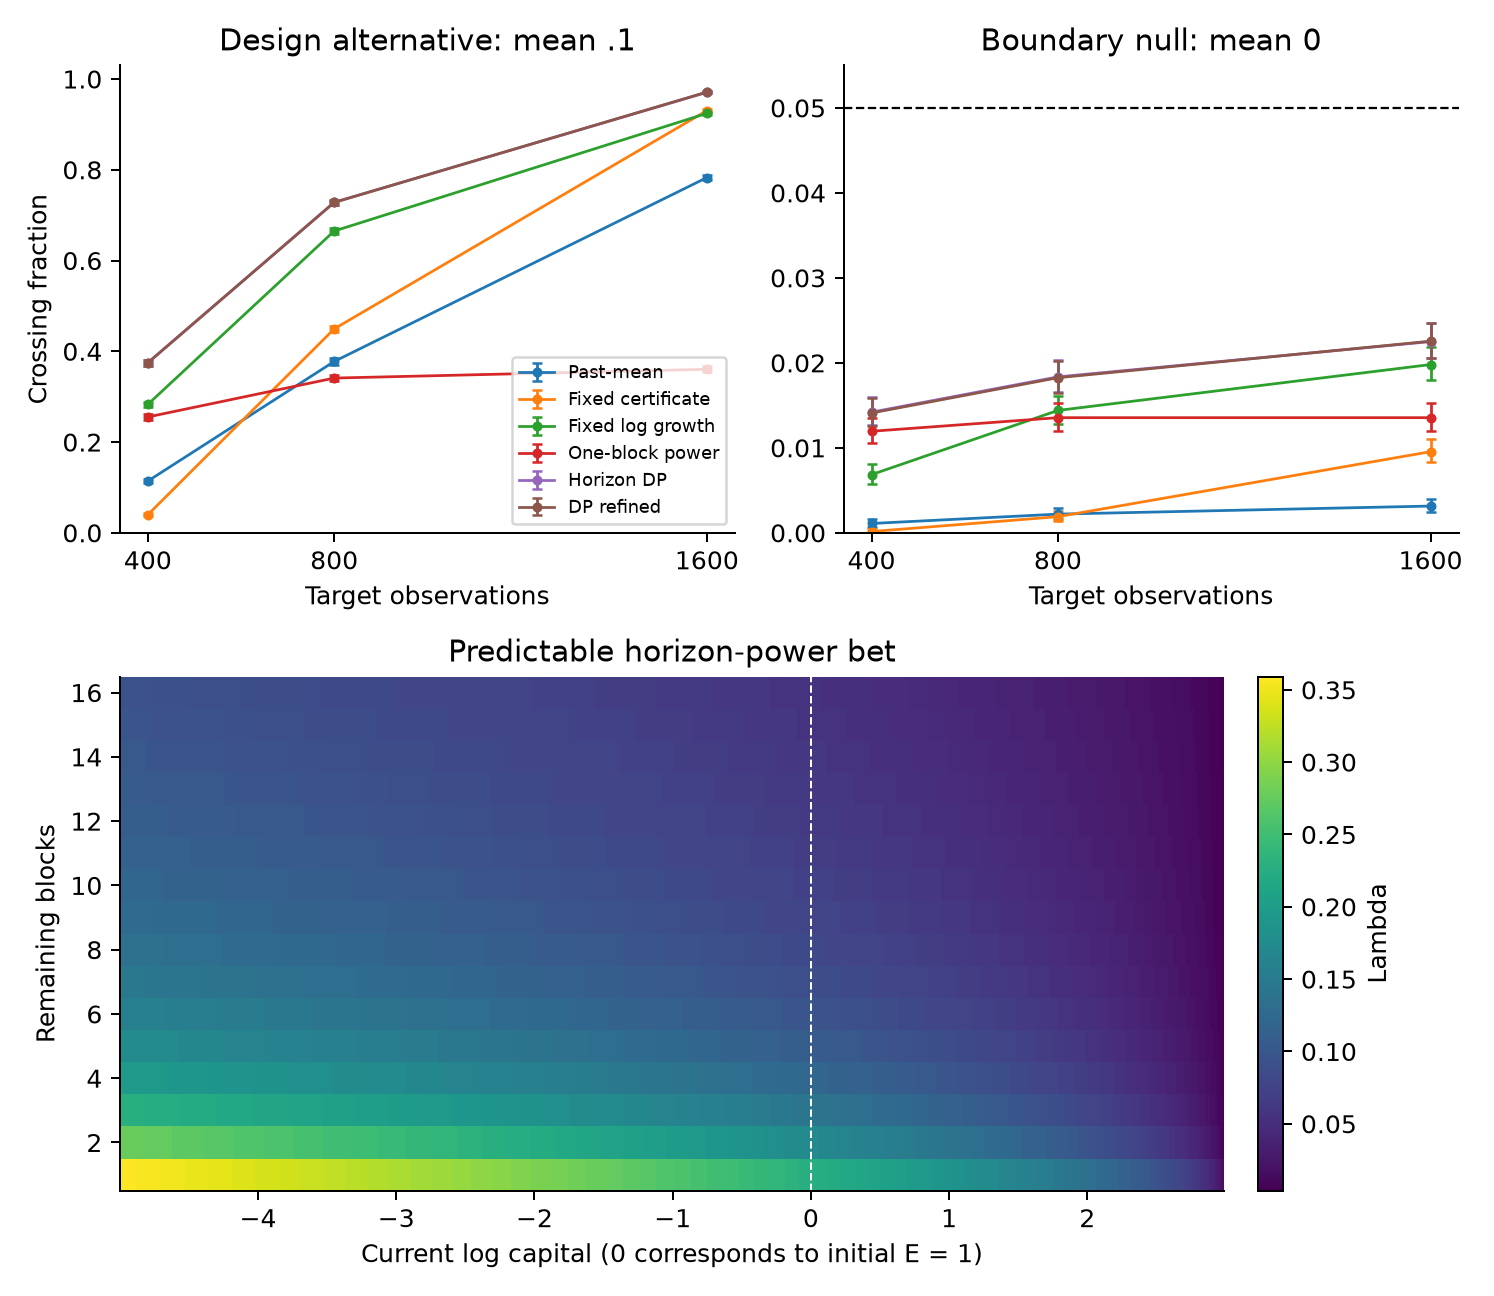
\includegraphics[width=.97\linewidth]{figures/lambda_power.png}

\caption{Top: observed design-power and null-crossing fractions with pointwise Wilson 95\% intervals. Each DP point uses its own target horizon; the connected points are not one policy monitored at three dates. Bottom: the primary working-model bet as a function of pre-block log capital and remaining blocks. Bets and decisions share the 100-observation calendar.}\label{fig:lambda-power}\end{figure}

\subsection{A fresh comparison with a deadline-optimized constant}

The first experiment compares the Bellman rule with certificate and log-growth bets, which target different objectives. To separate deadline calibration from adaptation to evidence, a new companion experiment chooses the best constant stake on each existing action grid for each deadline. It maximizes working-model probability of crossing at a review, using a constant-action recursion rather than the Bellman maximum at each state. Stake selection and source hashes are frozen before drawing the fresh seed-450001 stream. This is an explicitly subsequent comparison, not an additional arm fitted to the first experiment or extra replications of its paths.

Writing $W_0^\lambda=V_0$, the constant-action recursion is $W_k^\lambda(\ell)=1$ for $\ell\ge b_\alpha$, and $W_k^\lambda(\ell)=\int W_{k-1}^\lambda(\ell+z)Q_\lambda(dz)$ otherwise. The selected constant maximizes $W_H^\lambda(0)$ over the grid actions, rather than taking a new maximum at every state.

Both grids select the same three constant bets. Their predicted maximum powers differ by at most 0.000465. The fixed-arm simulation holds its stake until crossing or its own deadline, including below the computational lower boundary; absorption there is only a numerical approximation in its value calculation. All twelve predicted-versus-observed DP/constant design-power checks pass the same declared numerical-plus-Monte-Carlo tolerance.

\begin{table}[H]\centering\small

\begin{tabular}{rrrrrl}\toprule

Deadline & Constant $\lambda$ & Constant (\%) & Horizon DP (\%) & Gain (pp) & 95\% MC interval \\\midrule

400 & 0.12721 & 33.10 & 37.35 & 4.26 & [3.96, 4.55] \\

800 & 0.08980 & 66.02 & 72.71 & 6.70 & [6.33, 7.06] \\

1600 & 0.06361 & 94.42 & 96.76 & 2.34 & [2.12, 2.56] \\

\bottomrule\end{tabular}

\caption{Fresh companion comparison at actual mean .1, with 20,000 paired paths, the unchanged nominal individual 5\% bound, and the common betting/review calendar. Constants maximize horizon power on the declared working-model action grid. Each deadline uses its own two policies. Gain intervals are pointwise paired normal-approximation Monte Carlo intervals, unadjusted across comparisons; this is not matched-actual-size inference.}\label{tab:constant-power}\end{table}

At 400 observations the counts are 7470/20000 for horizon DP and 6619/20000 for the optimized constant. The corresponding null fractions are 1.29\% and 1.04\%. Thus the gain is beyond selecting one better constant at the common nominal level; actual null rejection probabilities remain different. Both numerical resolutions, the unchanged earlier comparators and actual means .2 and .3 are retained in the report. Original and companion powers are reported separately and are not pooled.

The independent companion audit reconstructs every DP/fixed stake and every first crossing (20,497,504 scalar checks). Direct multiplicative score replay covers sixteen paths per law and has maximum log-capital discrepancy 8.88e-14; it is not a replay of every score path. This comparison supplies neither a continuous-action global optimum nor a financial performance claim.

\paragraph{A Gaussian power envelope.}

The classical Neyman--Pearson bound \cite{neymanpearson} also applies to early rejection by a fixed deadline. For iid $N(0,\sigma^2)$ versus $N(\delta,\sigma^2)$, $\delta>0$, any test with actual null rejection probability $s$ by $H$ has power at most

\[B_H(s)=\Phi\!\left(\delta\sqrt H/\sigma+\Phi^{-1}(s)\right).\]

Indeed, its rejection event is measurable from the first $H$ scores; their likelihood ratio is increasing in their sum. A terminal upper-tail sum test maximizes power at size $s$, giving the formula. Independent test randomization does not improve this bound. This oracle fixes the two Gaussian laws: its attaining test need not be valid over the full moment null or under unrestricted monitoring.

At the design alternative, $B_H(.05)$ is 63.88\%, 88.17\%, 99.07\% at the three deadlines. Substituting the observed null fractions of the fresh primary DP rules gives descriptive values 40.94\%, 77.12\%, 97.60\%. These plug-ins do not determine the true null sizes or establish matched-size dominance. The post-hoc report retains both grids, both rule classes and all three alternatives, and gives simultaneous exact-binomial uncertainty limits. It uses the existing audited counts without new paths, threshold changes or policy selection.

